% Options for packages loaded elsewhere
\PassOptionsToPackage{unicode}{hyperref}
\PassOptionsToPackage{hyphens}{url}
%
\documentclass[
]{krantz}
\usepackage{amsmath,amssymb}
\usepackage{iftex}
\ifPDFTeX
  \usepackage[T1]{fontenc}
  \usepackage[utf8]{inputenc}
  \usepackage{textcomp} % provide euro and other symbols
\else % if luatex or xetex
  \usepackage{unicode-math} % this also loads fontspec
  \defaultfontfeatures{Scale=MatchLowercase}
  \defaultfontfeatures[\rmfamily]{Ligatures=TeX,Scale=1}
\fi
\usepackage{lmodern}
\ifPDFTeX\else
  % xetex/luatex font selection
\fi
% Use upquote if available, for straight quotes in verbatim environments
\IfFileExists{upquote.sty}{\usepackage{upquote}}{}
\IfFileExists{microtype.sty}{% use microtype if available
  \usepackage[]{microtype}
  \UseMicrotypeSet[protrusion]{basicmath} % disable protrusion for tt fonts
}{}
\makeatletter
\@ifundefined{KOMAClassName}{% if non-KOMA class
  \IfFileExists{parskip.sty}{%
    \usepackage{parskip}
  }{% else
    \setlength{\parindent}{0pt}
    \setlength{\parskip}{6pt plus 2pt minus 1pt}}
}{% if KOMA class
  \KOMAoptions{parskip=half}}
\makeatother
\usepackage{xcolor}
\usepackage{color}
\usepackage{fancyvrb}
\newcommand{\VerbBar}{|}
\newcommand{\VERB}{\Verb[commandchars=\\\{\}]}
\DefineVerbatimEnvironment{Highlighting}{Verbatim}{commandchars=\\\{\}}
% Add ',fontsize=\small' for more characters per line
\usepackage{framed}
\definecolor{shadecolor}{RGB}{248,248,248}
\newenvironment{Shaded}{\begin{snugshade}}{\end{snugshade}}
\newcommand{\AlertTok}[1]{\textcolor[rgb]{0.94,0.16,0.16}{#1}}
\newcommand{\AnnotationTok}[1]{\textcolor[rgb]{0.56,0.35,0.01}{\textbf{\textit{#1}}}}
\newcommand{\AttributeTok}[1]{\textcolor[rgb]{0.13,0.29,0.53}{#1}}
\newcommand{\BaseNTok}[1]{\textcolor[rgb]{0.00,0.00,0.81}{#1}}
\newcommand{\BuiltInTok}[1]{#1}
\newcommand{\CharTok}[1]{\textcolor[rgb]{0.31,0.60,0.02}{#1}}
\newcommand{\CommentTok}[1]{\textcolor[rgb]{0.56,0.35,0.01}{\textit{#1}}}
\newcommand{\CommentVarTok}[1]{\textcolor[rgb]{0.56,0.35,0.01}{\textbf{\textit{#1}}}}
\newcommand{\ConstantTok}[1]{\textcolor[rgb]{0.56,0.35,0.01}{#1}}
\newcommand{\ControlFlowTok}[1]{\textcolor[rgb]{0.13,0.29,0.53}{\textbf{#1}}}
\newcommand{\DataTypeTok}[1]{\textcolor[rgb]{0.13,0.29,0.53}{#1}}
\newcommand{\DecValTok}[1]{\textcolor[rgb]{0.00,0.00,0.81}{#1}}
\newcommand{\DocumentationTok}[1]{\textcolor[rgb]{0.56,0.35,0.01}{\textbf{\textit{#1}}}}
\newcommand{\ErrorTok}[1]{\textcolor[rgb]{0.64,0.00,0.00}{\textbf{#1}}}
\newcommand{\ExtensionTok}[1]{#1}
\newcommand{\FloatTok}[1]{\textcolor[rgb]{0.00,0.00,0.81}{#1}}
\newcommand{\FunctionTok}[1]{\textcolor[rgb]{0.13,0.29,0.53}{\textbf{#1}}}
\newcommand{\ImportTok}[1]{#1}
\newcommand{\InformationTok}[1]{\textcolor[rgb]{0.56,0.35,0.01}{\textbf{\textit{#1}}}}
\newcommand{\KeywordTok}[1]{\textcolor[rgb]{0.13,0.29,0.53}{\textbf{#1}}}
\newcommand{\NormalTok}[1]{#1}
\newcommand{\OperatorTok}[1]{\textcolor[rgb]{0.81,0.36,0.00}{\textbf{#1}}}
\newcommand{\OtherTok}[1]{\textcolor[rgb]{0.56,0.35,0.01}{#1}}
\newcommand{\PreprocessorTok}[1]{\textcolor[rgb]{0.56,0.35,0.01}{\textit{#1}}}
\newcommand{\RegionMarkerTok}[1]{#1}
\newcommand{\SpecialCharTok}[1]{\textcolor[rgb]{0.81,0.36,0.00}{\textbf{#1}}}
\newcommand{\SpecialStringTok}[1]{\textcolor[rgb]{0.31,0.60,0.02}{#1}}
\newcommand{\StringTok}[1]{\textcolor[rgb]{0.31,0.60,0.02}{#1}}
\newcommand{\VariableTok}[1]{\textcolor[rgb]{0.00,0.00,0.00}{#1}}
\newcommand{\VerbatimStringTok}[1]{\textcolor[rgb]{0.31,0.60,0.02}{#1}}
\newcommand{\WarningTok}[1]{\textcolor[rgb]{0.56,0.35,0.01}{\textbf{\textit{#1}}}}
\usepackage{longtable,booktabs,array}
\usepackage{calc} % for calculating minipage widths
% Correct order of tables after \paragraph or \subparagraph
\usepackage{etoolbox}
\makeatletter
\patchcmd\longtable{\par}{\if@noskipsec\mbox{}\fi\par}{}{}
\makeatother
% Allow footnotes in longtable head/foot
\IfFileExists{footnotehyper.sty}{\usepackage{footnotehyper}}{\usepackage{footnote}}
\makesavenoteenv{longtable}
\usepackage{graphicx}
\makeatletter
\def\maxwidth{\ifdim\Gin@nat@width>\linewidth\linewidth\else\Gin@nat@width\fi}
\def\maxheight{\ifdim\Gin@nat@height>\textheight\textheight\else\Gin@nat@height\fi}
\makeatother
% Scale images if necessary, so that they will not overflow the page
% margins by default, and it is still possible to overwrite the defaults
% using explicit options in \includegraphics[width, height, ...]{}
\setkeys{Gin}{width=\maxwidth,height=\maxheight,keepaspectratio}
% Set default figure placement to htbp
\makeatletter
\def\fps@figure{htbp}
\makeatother
\setlength{\emergencystretch}{3em} % prevent overfull lines
\providecommand{\tightlist}{%
  \setlength{\itemsep}{0pt}\setlength{\parskip}{0pt}}
\setcounter{secnumdepth}{5}
\usepackage[portuguese]{babel}

\usepackage{booktabs}
\usepackage{longtable}
\usepackage[bf,singlelinecheck=off]{caption}

\usepackage{Alegreya}
\usepackage[scale=.7]{sourcecodepro}

\usepackage{framed,color}
\definecolor{shadecolor}{RGB}{248,248,248}

\renewcommand{\textfraction}{0.05}
\renewcommand{\topfraction}{0.8}
\renewcommand{\bottomfraction}{0.8}
\renewcommand{\floatpagefraction}{0.75}

\renewenvironment{quote}{\begin{VF}}{\end{VF}}
\usepackage{hyperref}
\let\oldhref\href
\renewcommand{\href}[2]{#2\footnote{\url{#1}}}

\ifxetex
  \usepackage{letltxmacro}
  \setlength{\XeTeXLinkMargin}{1pt}
  \LetLtxMacro\SavedIncludeGraphics\includegraphics
  \def\includegraphics#1#{% #1 catches optional stuff (star/opt. arg.)
    \IncludeGraphicsAux{#1}%
  }%
  \newcommand*{\IncludeGraphicsAux}[2]{%
    \XeTeXLinkBox{%
      \SavedIncludeGraphics#1{#2}%
    }%
  }%
\fi

\makeatletter
\newenvironment{kframe}{%
\medskip{}
\setlength{\fboxsep}{.8em}
 \def\at@end@of@kframe{}%
 \ifinner\ifhmode%
  \def\at@end@of@kframe{\end{minipage}}%
  \begin{minipage}{\columnwidth}%
 \fi\fi%
 \def\FrameCommand##1{\hskip\@totalleftmargin \hskip-\fboxsep
 \colorbox{shadecolor}{##1}\hskip-\fboxsep
     % There is no \\@totalrightmargin, so:
     \hskip-\linewidth \hskip-\@totalleftmargin \hskip\columnwidth}%
 \MakeFramed {\advance\hsize-\width
   \@totalleftmargin\z@ \linewidth\hsize
   \@setminipage}}%
 {\par\unskip\endMakeFramed%
 \at@end@of@kframe}
\makeatother

\makeatletter
\@ifundefined{Shaded}{
}{\renewenvironment{Shaded}{\begin{kframe}}{\end{kframe}}}
\makeatother

\newenvironment{rmdblock}[1]
  {
  \begin{itemize}
  \renewcommand{\labelitemi}{
    \raisebox{-.7\height}[0pt][0pt]{
      {\setkeys{Gin}{width=3em,keepaspectratio}\includegraphics{images/#1}}
    }
  }
  \setlength{\fboxsep}{1em}
  \begin{kframe}
  \item
  }
  {
  \end{kframe}
  \end{itemize}
  }
\newenvironment{rmdnote}
  {\begin{rmdblock}{note}}
  {\end{rmdblock}}
\newenvironment{rmdcaution}
  {\begin{rmdblock}{caution}}
  {\end{rmdblock}}
\newenvironment{rmdimportant}
  {\begin{rmdblock}{important}}
  {\end{rmdblock}}
\newenvironment{rmdtip}
  {\begin{rmdblock}{tip}}
  {\end{rmdblock}}
\newenvironment{rmdwarning}
  {\begin{rmdblock}{warning}}
  {\end{rmdblock}}

\usepackage{makeidx}
\makeindex

\urlstyle{tt}

\usepackage{amsthm}
\makeatletter
\def\thm@space@setup{%
  \thm@preskip=8pt plus 2pt minus 4pt
  \thm@postskip=\thm@preskip
}
\makeatother

\frontmatter
\ifLuaTeX
  \usepackage{selnolig}  % disable illegal ligatures
\fi
\usepackage[]{natbib}
\bibliographystyle{plainnat}
\IfFileExists{bookmark.sty}{\usepackage{bookmark}}{\usepackage{hyperref}}
\IfFileExists{xurl.sty}{\usepackage{xurl}}{} % add URL line breaks if available
\urlstyle{same}
\hypersetup{
  pdftitle={R para Data Science},
  pdfauthor={Jeidsan A. da C. Pereira},
  hidelinks,
  pdfcreator={LaTeX via pandoc}}

\title{R para Data Science}
\usepackage{etoolbox}
\makeatletter
\providecommand{\subtitle}[1]{% add subtitle to \maketitle
  \apptocmd{\@title}{\par {\large #1 \par}}{}{}
}
\makeatother
\subtitle{Solução dos exercícios}
\author{Jeidsan A. da C. Pereira}
\date{2023-10-25}

\usepackage{amsthm}
\newtheorem{theorem}{Teorema}[chapter]
\newtheorem{lemma}{Lema}[chapter]
\newtheorem{corollary}{Corolário}[chapter]
\newtheorem{proposition}{Proposição}[chapter]
\newtheorem{conjecture}{Conjectura}[chapter]
\theoremstyle{definition}
\newtheorem{definition}{Definição}[chapter]
\theoremstyle{definition}
\newtheorem{example}{Exemplo}[chapter]
\theoremstyle{definition}
\newtheorem{exercise}{Exercício}[chapter]
\theoremstyle{definition}
\newtheorem{hypothesis}{Hipótese}[chapter]
\theoremstyle{remark}
\newtheorem*{remark}{Observação}
\newtheorem*{solution}{Solução}
\begin{document}
\maketitle

%\cleardoublepage\newpage\thispagestyle{empty}\null
%\cleardoublepage\newpage\thispagestyle{empty}\null
%\cleardoublepage\newpage
\thispagestyle{empty}
\begin{center}
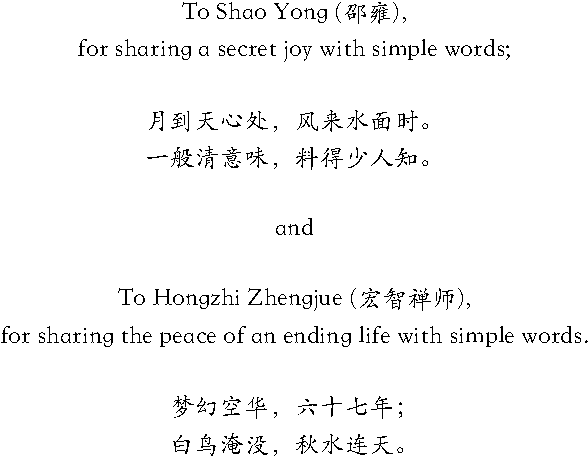
\includegraphics{images/dedication.pdf}
\end{center}

\setlength{\abovedisplayskip}{-5pt}
\setlength{\abovedisplayshortskip}{-5pt}

{
\setcounter{tocdepth}{1}
\tableofcontents
}
\hypertarget{prefuxe1cio}{%
\chapter*{Prefácio}\label{prefuxe1cio}}
\addcontentsline{toc}{chapter}{Prefácio}

Esta página serviu para estudo e prática com o pacote R Bookdown e contém a solução encontrada por mim para os exercícios propostos no livro R para Data Sciente, de Hadley Wickham e Garret Grolemund, publicado no Brasil em 2019 pela Alta Books Editora \citep{wickham2019}.

Por se tratar de um produto construído durante o processo de aprendizagem, o conteúdo pode conter erros, tanto no texto em si, como na lógica utilizada para solução dos exercícios.

Dúvidas ou sugestões de melhoria podem ser encaminhadas para o e-mail \emph{\href{mailto:jeidsan.pereira@gmail.com}{\nolinkurl{jeidsan.pereira@gmail.com}}}.

\mainmatter

\hypertarget{part-explorar}{%
\part{Explorar}\label{part-explorar}}

\hypertarget{visualizauxe7uxe3o-de-dados-com-ggplot2}{%
\chapter{\texorpdfstring{Visualização de dados com \texttt{ggplot2}}{Visualização de dados com ggplot2}}\label{visualizauxe7uxe3o-de-dados-com-ggplot2}}

Para a correta execução dos códigos desse capítulo, utilizaremos algumas configurações específicas.

Inicialmente, precisaremos carregar o pacote \texttt{nycflights13}, que contém os dados de todos os voos da cidade de Nova York em 2013.

\begin{Shaded}
\begin{Highlighting}[]
\FunctionTok{library}\NormalTok{(nycflights13)}
\end{Highlighting}
\end{Shaded}

\hypertarget{introduuxe7uxe3o}{%
\section{Introdução}\label{introduuxe7uxe3o}}

Não temos exercícios nesta seção.

\hypertarget{primeiros-passos}{%
\section{Primeiros passos}\label{primeiros-passos}}

\hypertarget{exr1-2-1}{%
\subsection*{Exercício 1.2.1}\label{exr1-2-1}}
\addcontentsline{toc}{subsection}{Exercício 1.2.1}

Execute \texttt{ggplot(data=mpg);}. O que você vê?

\begin{solution}
\leavevmode

\begin{Shaded}
\begin{Highlighting}[]
\FunctionTok{ggplot}\NormalTok{(}\AttributeTok{data=}\NormalTok{mpg) }\SpecialCharTok{+}
\NormalTok{    tema}
\end{Highlighting}
\end{Shaded}


\includegraphics{r4ds_files/figure-latex/unnamed-chunk-3-1.pdf}

É exibido um quadro em branco. Este quadro contém o sistema de coordenadas sobre o qual serão desenhados os grpaficos que pretendemos exibir.

\end{solution}

\hypertarget{exr1-2-2}{%
\subsection*{Exercício 1.2.2}\label{exr1-2-2}}
\addcontentsline{toc}{subsection}{Exercício 1.2.2}

Quantas linhas existem em \texttt{mtcars}? Quantas colunas?

\begin{solution}
\leavevmode

\begin{Shaded}
\begin{Highlighting}[]
\FunctionTok{dim}\NormalTok{(mtcars)}
\end{Highlighting}
\end{Shaded}

\begin{verbatim}
## [1] 32 11
\end{verbatim}

R.: Existem 32 linhas e 11 colunas.

\end{solution}

\hypertarget{exr1-2-3}{%
\subsection*{Exercício 1.2.3}\label{exr1-2-3}}
\addcontentsline{toc}{subsection}{Exercício 1.2.3}

O que a variável \texttt{drv} descreve?

\begin{solution}
Executamos o comando \texttt{?mpg} no console no R e a página de ajuda foi aberta. Nela encontramos o significado de cada variável do conjunto de dados.

A varíável descreve o tipo de tração dos carros analisados, onde \texttt{f} significa tração dianteira, \texttt{r} significa tração traseira e \texttt{4} significa tração nas quatro rodas.
\end{solution}

\hypertarget{ex1-2-4}{%
\subsection*{Exercício 1.2.4}\label{ex1-2-4}}
\addcontentsline{toc}{subsection}{Exercício 1.2.4}

Faça um gráfico de dispersão de \texttt{hwy} \emph{versus} \texttt{cyl}.

\begin{solution}
\leavevmode

\begin{Shaded}
\begin{Highlighting}[]
\FunctionTok{ggplot}\NormalTok{(}\AttributeTok{data =}\NormalTok{ mpg) }\SpecialCharTok{+}
    \FunctionTok{geom\_point}\NormalTok{(}\AttributeTok{mapping =} \FunctionTok{aes}\NormalTok{(}\AttributeTok{x =}\NormalTok{ hwy, }\AttributeTok{y =}\NormalTok{ cyl)) }\SpecialCharTok{+}
\NormalTok{    tema}
\end{Highlighting}
\end{Shaded}

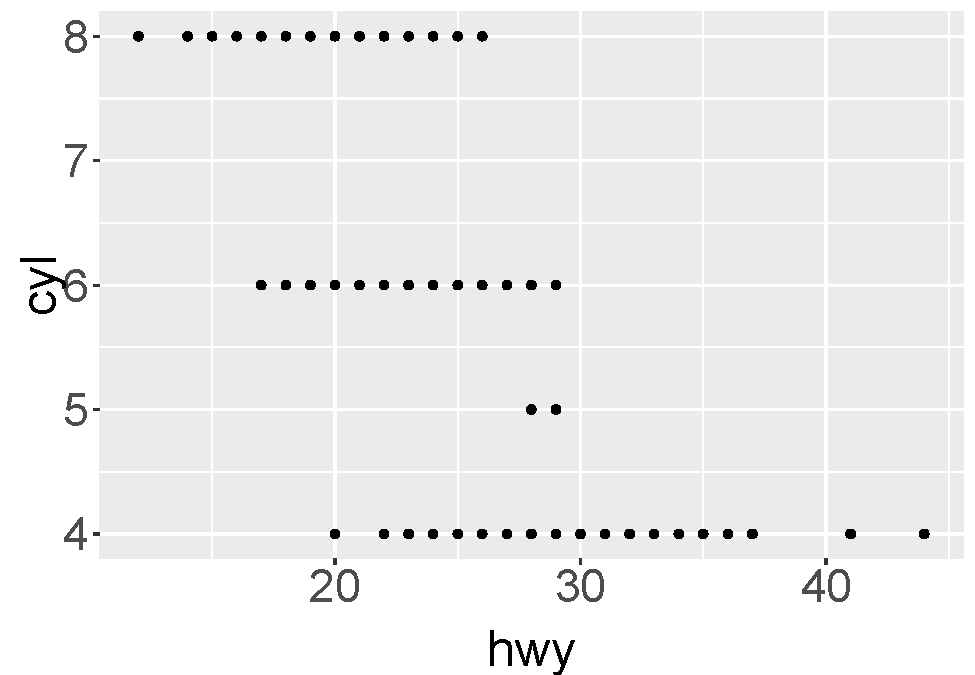
\includegraphics{r4ds_files/figure-latex/unnamed-chunk-5-1.pdf}

\end{solution}

\hypertarget{mapeamentos-estuxe9ticos}{%
\section{Mapeamentos estéticos}\label{mapeamentos-estuxe9ticos}}

\hypertarget{exr1-3-1}{%
\subsection*{Exercício 1.3.1}\label{exr1-3-1}}
\addcontentsline{toc}{subsection}{Exercício 1.3.1}

\begin{exercise}
x
\end{exercise}

\begin{solution}
x
\end{solution}

\hypertarget{problemas-comuns}{%
\section{Problemas comuns}\label{problemas-comuns}}

\begin{exercise}
x
\end{exercise}

\hypertarget{facetas}{%
\section{Facetas}\label{facetas}}

\begin{exercise}
x
\end{exercise}

\hypertarget{objetos-geomuxe9tricos}{%
\section{Objetos geométricos}\label{objetos-geomuxe9tricos}}

\begin{exercise}
x
\end{exercise}

\hypertarget{transformauxe7uxf5es-estatuxedsticas}{%
\section{Transformações estatísticas}\label{transformauxe7uxf5es-estatuxedsticas}}

\begin{exercise}
x
\end{exercise}

\hypertarget{ajustes-de-posiuxe7uxe3o}{%
\section{Ajustes de posição}\label{ajustes-de-posiuxe7uxe3o}}

\begin{exercise}
x
\end{exercise}

\hypertarget{sistemas-de-coordenadas}{%
\section{Sistemas de coordenadas}\label{sistemas-de-coordenadas}}

\begin{exercise}
x
\end{exercise}

\hypertarget{a-gramuxe1tica-em-camadas-de-gruxe1ficos}{%
\section{A gramática em camadas de gráficos}\label{a-gramuxe1tica-em-camadas-de-gruxe1ficos}}

\begin{exercise}
x
\end{exercise}

\hypertarget{fluxo-de-trabalho-o-buxe1sico}{%
\chapter{Fluxo de trabalho: o básico}\label{fluxo-de-trabalho-o-buxe1sico}}

\hypertarget{transformauxe7uxe3o-de-dados-com-dplyr}{%
\chapter{\texorpdfstring{Transformação de dados com \texttt{dplyr}}{Transformação de dados com dplyr}}\label{transformauxe7uxe3o-de-dados-com-dplyr}}

\hypertarget{fluxo-de-trabalho-scripts}{%
\chapter{Fluxo de trabalho: scripts}\label{fluxo-de-trabalho-scripts}}

\hypertarget{anuxe1lise-exploratuxf3ria-de-dados}{%
\chapter{Análise exploratória de dados}\label{anuxe1lise-exploratuxf3ria-de-dados}}

\hypertarget{fluxo-de-trabalho-projetos}{%
\chapter{Fluxo de trabalho: projetos}\label{fluxo-de-trabalho-projetos}}

\hypertarget{part-wrangle}{%
\part{Wrangle}\label{part-wrangle}}

\hypertarget{tibbles-com-tibble}{%
\chapter{\texorpdfstring{Tibbles com \texttt{tibble}}{Tibbles com tibble}}\label{tibbles-com-tibble}}

\hypertarget{importando-dados-com-readr}{%
\chapter{\texorpdfstring{Importando dados com \texttt{readr}}{Importando dados com readr}}\label{importando-dados-com-readr}}

\hypertarget{arrumando-dados-com-tidyr}{%
\chapter{\texorpdfstring{Arrumando dados com \texttt{tidyr}}{Arrumando dados com tidyr}}\label{arrumando-dados-com-tidyr}}

\hypertarget{dados-relacionais-com-dplyr}{%
\chapter{\texorpdfstring{Dados relacionais com \texttt{dplyr}}{Dados relacionais com dplyr}}\label{dados-relacionais-com-dplyr}}

\hypertarget{strings-com-stringr}{%
\chapter{\texorpdfstring{Strings com \texttt{stringr}}{Strings com stringr}}\label{strings-com-stringr}}

\hypertarget{fatores-com-forcats}{%
\chapter{\texorpdfstring{Fatores com \texttt{forcats}}{Fatores com forcats}}\label{fatores-com-forcats}}

\hypertarget{datas-e-horas-com-lubridate}{%
\chapter{\texorpdfstring{Datas e horas com \texttt{lubridate}}{Datas e horas com lubridate}}\label{datas-e-horas-com-lubridate}}

\hypertarget{part-programar}{%
\part{Programar}\label{part-programar}}

\hypertarget{pipes-com-magrittr}{%
\chapter{\texorpdfstring{Pipes com \texttt{magrittr}}{Pipes com magrittr}}\label{pipes-com-magrittr}}

\hypertarget{funuxe7uxf5es}{%
\chapter{Funções}\label{funuxe7uxf5es}}

\hypertarget{vetores}{%
\chapter{Vetores}\label{vetores}}

\hypertarget{iterauxe7uxe3o-com-purrr}{%
\chapter{\texorpdfstring{Iteração com \texttt{purrr}}{Iteração com purrr}}\label{iterauxe7uxe3o-com-purrr}}

\hypertarget{part-modelar}{%
\chapter{(PART) Modelar}\label{part-modelar}}

\hypertarget{o-buxe1sico-de-modelos-com-modelr}{%
\chapter{\texorpdfstring{O básico de modelos com \texttt{modelr}}{O básico de modelos com modelr}}\label{o-buxe1sico-de-modelos-com-modelr}}

\hypertarget{construuxe7uxe3o-de-modelos}{%
\chapter{Construção de modelos}\label{construuxe7uxe3o-de-modelos}}

\hypertarget{muitos-modelos-com-purrr-e-broom}{%
\chapter{\texorpdfstring{Muitos modelos com \texttt{purrr} e \texttt{broom}}{Muitos modelos com purrr e broom}}\label{muitos-modelos-com-purrr-e-broom}}

\hypertarget{part-comunicar}{%
\part{Comunicar}\label{part-comunicar}}

\hypertarget{r-markdown}{%
\chapter{R Markdown}\label{r-markdown}}

\hypertarget{gruxe1ficos-para-comunicauxe7uxe3o-com-ggplot2}{%
\chapter{\texorpdfstring{Gráficos para comunicação com \texttt{ggplot2}}{Gráficos para comunicação com ggplot2}}\label{gruxe1ficos-para-comunicauxe7uxe3o-com-ggplot2}}

\hypertarget{formatos-r-markdown}{%
\chapter{Formatos R Markdown}\label{formatos-r-markdown}}

\hypertarget{fluxo-de-trabalho-de-r-markdown}{%
\chapter{Fluxo de trabalho de R Markdown}\label{fluxo-de-trabalho-de-r-markdown}}

  \bibliography{book.bib,packages.bib}

\printindex

\end{document}
